\documentclass[PianoDiQualifica.tex]{subfiles}

\begin{document}
%http://www.praxiom.com/iso-90003.htm citato da Tullio può servire come base per capire processi meglio
\chapter{Qualità di processo}

\section{Scopo} 
Per garantire la qualità del prodotto è necessario perseguire la qualità dei processi che lo definiscono.
Per raggiungere questo obiettivo, si è deciso di seguire il principio di miglioramento continuo (PDCA) e di adottare lo standard ISO/IEC 15504 denominato SPICE (Software Process Improvement and Capability Determination).

\section{Procedure di controllo di qualità di processo}
La qualità dei processi verrà garantita dall'applicazione del principio PDCA, descritto dell'appendice A. Grazie a questo principio, sarà possibile ottenere un miglioramento continuo della qualità di tutti i processi, inclusa la verifica, e come diretta conseguenza si otterrà il miglioramento dei prodotti risultanti. 

Per ottenere qualità dei processi, bisogna:
\begin{itemize}
	\item Definire il processo: affinché sia controllabile;
	\item Controllare il processo: in funzione dell'ottenimento di efficacia, efficienza ed esperienza;
	\item Usare buoni strumenti di valutazione: SPICE e PDCA;
\end{itemize}

\section{Metriche per i processi}

\subsection{Schedule Variance (SV)}
Indica se si è in linea, in anticipo o in ritardo rispetto alla schedulazione delle attività di progetto pianificate nella baseline.\\
È un indicatore di efficacia soprattutto nei confronti del Cliente. \\
Se SV è positivo, significa che il progetto sta producendo con maggior velocità rispetto a quanto pianificato, viceversa se negativo.


\subsection{Budget Variance (BV)}
Indica se alla data corrente si è speso di più o di meno rispetto a quanto previsto a budget alla data corrente.\\
È un indicatore che ha un valore unicamente contabile e finanziario.\\
Se BV è positivo significa che il progetto sta spendendo il proprio budget con minor velocità di quanto pianificato, viceversa se negativo.


\begin{appendices}

\chapter{Ciclo di Deming o PDCA}
Ogni processo deve essere organizzato basandosi sul principio del miglioramento continuo (o ruota di Deming):
\begin{description}
	\item [Plan] (pianificare): viene definito un piano che parte dalla definizione di problemi e obiettivi, pianifica compiti, assegna responsabilità, studia il caso, analizza le cause della criticità, definisce azioni correttive; 
	\item [Do](eseguire): vengono implementate le attività secondo le linee definite durante la fase Plan;
	\item [Check] (valutare): viene verificato l'esito delle azioni di miglioramento rispetto alle attese;
	\item [Act] (agire): vengono applicate le correzioni necessarie per colmare le carenze rilevate, e vengono standardizzate le attività correttamente eseguite.
\end{description}

\begin{figure}[htbp]
	\begin{center}
		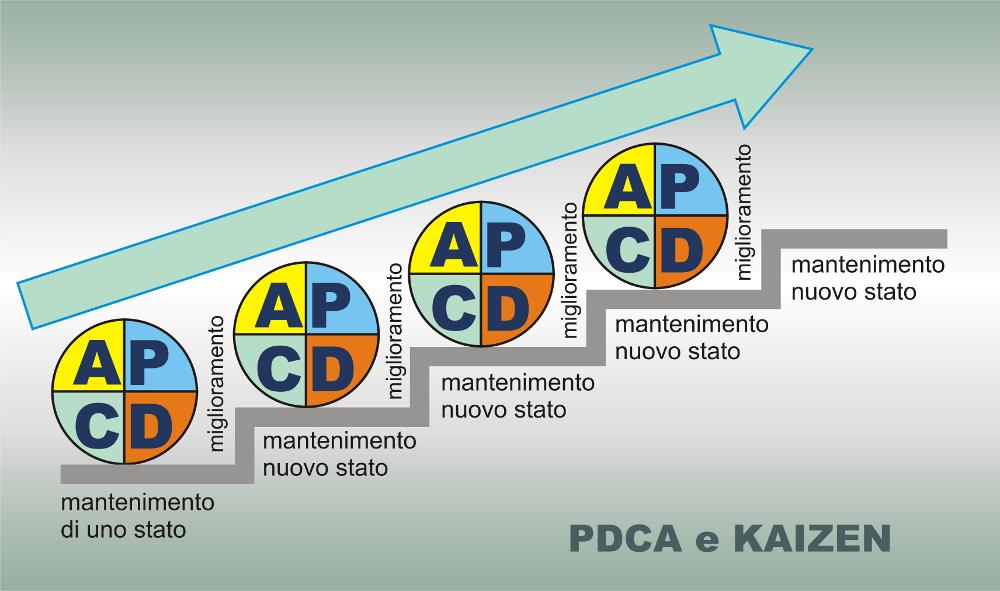
\includegraphics[width=0.7\linewidth]{../../common/images/PDCAkaizen}
		\caption[Ciclo di Deming]{Ciclo di Deming}
		\label{fig:pdca}
	\end{center}
\end{figure}

\chapter{ISO/IEC 15504}
Lo standard ISO/IEC 15504 contiene un modello di riferimento che definisce 
\begin{itemize}
	\item Process dimension;
	\item Capability dimension.
\end{itemize}

La dimensione di processo divide i processi in cinque categorie:
\begin{itemize}
	\item Customer-supplier;
	\item Engineering;
	\item Supporting;
	\item Management;
	\item Organization.
\end{itemize}

Per ogni processo, lo standard ISO/IEC 15504 definisce dei livelli di capacità:
\begin{description}
	\item [\normalfont Livello 5] \textbf{Optimizing process}: il processo è continuamente migliorato;
	\item [\normalfont Livello 4] \textbf{Predictable process}: il processo è adottato sistematicamente, entro limiti definiti;
	\item [\normalfont Livello 3] \textbf{Established process}: un processo stabilito si basa su un processo standard;
	\item [\normalfont Livello 2] \textbf{Managed process}: il processo è gestito e i prodotti sono stabiliti, controllati e mantenuti;
	\item [\normalfont Livello 1] \textbf{Performed process}: il processo è implementato e raggiunge lo scopo stabilito;
	\item [\normalfont Livello 0] \textbf{Incomplete process}: il processo non è implementato o non raggiunge lo scopo stabilito.\\
\end{description}

La capacità dei processi viene misurata attraverso degli attributi di processo.
\begin{description}
\item [Process performance:] capacità di un processo di raggiungere gli obiettivi trasformando input identificabili in output identificabili;
\item [Performance management:] capacità del processo di elaborare un prodotto coerente con gli obiettivi fissati;
\item [Work product management:] capacità del processo di elaborare un prodotto documentato, controllato e verificato;
\item [Process definition:] l'esecuzione del processo si basa su standard di processo per raggiungere i propri obiettivi;
\item [Process deployment:] capacità del processo di attingere a risorse tecniche e umane appropriate per essere attuato efficacemente;
\item [Process measurement:] gli obiettivi e le misure di prodotto e di processo vengono usati per garantire il raggiungimento dei traguardi definiti in supporto ai target aziendali;
\item [Process control:] il processo viene controllato tramite misure di prodotto e processo per effettuare correzioni migliorative al processo stesso;
\item [Process innovation:] i cambiamenti strutturali, di gestione e di esecuzione vengono gestiti in modo controllato per raggiungere i risultati fissati;
\item [Process optimization:] le modifiche al processo sono identificate e implementate per garantire il miglioramento continuo nella realizzazione degli obiettivi di business dell'organizzazione. 
\end{description}

Ogni attributo consiste di una o più pratiche generiche che sono ulteriormente elaborate in indicatori pratici per aiutare la valutazione delle performance, sotto forma di indici N-P-L-F:
\begin{itemize}
	\item Non soddisfatto (0 - 15\%);
	\item Parzialmente soddisfatto ($ > $15\% - 50\%);
	\item Largamente soddisfatto ($ > $50\% - 85\%);
	\item Totalmente soddisfatto ($ > $85\% - 100\%)
\end{itemize}

\end{appendices}
\end{document}